Assessing the chance of something happening in real life, one encounters more than just probabilities. It is directly connected to the model of our world, the probabilities of certain events happening inside the model, and how good the model actually resembles what we understand to be the truth. Models can be created using two trains of thought (xxx schools?) in statistics, about how to assign probabilities from observing events. Firstly, there is frequentist statistics, centered around the idea, that there is a fixed probability for an event that can, in theory, be derived from axioms[xxx]. Observing an event many times shall then directly converge towards the true value. Observe a coinflip as an example, the difference can be illustrated quite easily. If the coin is flipped often enough and the coin is fair, then we observe that every time the coin is flipped, the probabilities for observing "\textit{heads}" and "\textit{tails}" will converge another step towards $0.5$. 
\begin{figure}[h!]%Cloinflip
	\centering
	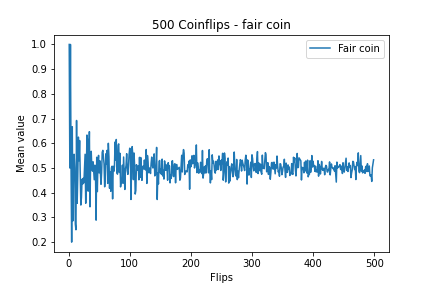
\includegraphics[width=4in]{img/05_1/fair_coinflip.png}
	\caption[Fair Coinflip]
	{A simulated fair coin flip, with 500 iterations of either \textit{heads} (1) or \textit{tails} (0). }
\end{figure}
If we repeat the experiment with an unfair coin instead, our assumption of a fair coin will now still lead us to assume the probabilities for \textit{heads} and \textit{tails} were $0.5$, just like in a perfect system. Here we are still assuming that if we observe enough events, the probabilities should be verified by the experiment. Statistical uncertainty in observing a fair coin could shift the observed probabilities for a while, but will always converge. Only after observing many events, we would start to question the assumptions we had at the beginning, e.g. of the coin being fair, because convergence is slow. 
\begin{figure}[h!]%Coinflip Comparison fair and unfair coin
	\centering
	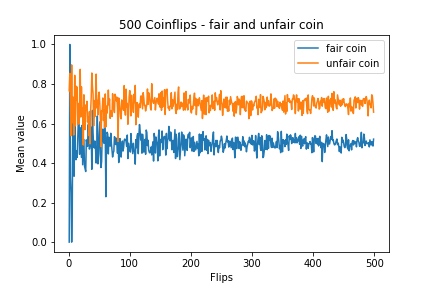
\includegraphics[width=4in]{img/05_1/unfair_coinflip.png}
	\caption[Fair and unfair coinflip comparison]
	{A simulated fair coin flip (blue) compared to the unfair coin flip (orange). Even though both tend towards different values for large sample sizes, in the first few flips, it is very hard to distinguish which coin is fair. Experimental conditions are the same as with the simulated fair coin flip.}
\end{figure}
So, from the frequentists perspective, if we were in the situation of playing coinflip with an unkown coin, it would take a long time, until we would accept the possibility that our model could be wrong. This inherent trust into the models is therefore used mostly in fields like physics, where the theory is assumed to reflect the ground truth no matter what, with the assumption that constants are always constant and the set of rules never changes, independent of where you are in the universe. This is called the Noether theorem, but since it only applies to the set of rules in physics, where controlling variables can be enforced with great precision, other fields need a more flexible theory to determine the probability of an event. So, assuming there are variables influencing our system in ways we cannot foresee with absolute precision, we need to be able to update the expected probabilities as a function of our observations. Since the probabilities are a crucial part of the model we applied to reality in the first place, we need to find a model that can be updated each time an observation took place. Bayesian statistics allows us to update our beliefs along the way. It dates back to Thomas Bayes, who in his essay "\textit{An essay towards solving a problem in the doctrine of chances}" [xxx] introduced the first version of this idea. Our percieved reality can always be flawed, not limited to a fair or unfair coin, but models for reality of all sorts can have intrinsic flaws, that can be quantified using this method of determining probabilities and updating models, along the way. Through this, probabilities become dependent on believability and credibility, confidence in decisions or environmental variables of the problem. Creating a model in bayesian statistics also allows for a causal bias introduced into the model, before observations even took place. So, if for example you would consider playing against someone with a coin you do not yet know to be fair, it is best to assume the coin is unfair at first. Noticing that a coin is unfair faster, and with higher probability, to update the model is valuable information. Previously we noticed, that the flexibility of bayesian models allow us to take into account environmental variables, but how many of those will actually lead to better predictions from the model? Occams Razor (xxx) is a good rule to follow, which would roughly translate to "\textit{choose a model as complicated as necessary but no more than that}". Or, in other words, a more complex model with more hyperparameters will in the end lead to better explanation ("a better fit") of the observed data, but prediction power will intrinsically decrease along the way, due to more noise being learned as a feature. 